\documentclass[11pt]{article}
\usepackage[margin=1in]{geometry}
\usepackage{booktabs}
\usepackage{array}
\usepackage{amsmath}
\usepackage{amssymb}
\usepackage{graphicx}
\usepackage{longtable}
\usepackage{lscape}
\usepackage[backend=biber,style=numeric,sorting=none]{biblatex}
\addbibresource{reference_update.bib}
\AtEveryBibitem{\clearfield{url}\clearfield{urlyear}\clearfield{urlmonth}\clearfield{urlday}\clearfield{note}\clearfield{keywords}\clearfield{abstract}\clearfield{issn}\clearfield{eprint}}
\renewcommand{\thetable}{S\arabic{table}}
\renewcommand{\thefigure}{S\arabic{figure}}
\raggedbottom
\makeatletter
\setlength{\@fptop}{0pt}
\makeatother

\title{Supplementary Material\\
Contrast-Level Aggregate-Data Dose--Response Meta-Analysis for Heterogeneous Exposure Intervals}
\author{Yangyifan Lu et al.}
\date{}

\begin{document}
\maketitle

\section*{Supplementary Methods S1: Regional distance-data construction}

To estimate the parameters $\alpha$ and $\theta$ of the Gamma distance
distribution, regional residential and animal-facility or agricultural-site location data were collected from
publicly available data. The eight studies included in the meta-analysis
covered four primary geographic regions: North Carolina, Wisconsin,
Pennsylvania, and the Netherlands. Among the Netherlands studies, most were
concentrated in Noord-Brabant and Limburg.

Publicly available spatial data for the U.S. regions were obtained from
ArcGIS, including residential census-block data and facility or site records.
Residential information was drawn from U.S. Census data, including population
and housing counts and geographic coordinates~\cite{US_Census}. The facility
classification schemes differed across state datasets and referred primarily
to animal species or production category. Categories most directly related to
animal-production exposures were retained; dairy- and egg-specific categories
were excluded when identifiable. North Carolina and Wisconsin used
permitted-facility layers~\cite{NC_CAFO,Wisconsin_cafo}. Pennsylvania used the
public CRAFT agricultural-producer directory, separated into dairy, egg, and
meat categories; it is not the Pennsylvania DEP CAFO permit layer and is
therefore a geospatial proxy~\cite{PA_CAFO,PA_DEP_CAFO}.
Spatial processing used ArcGIS Pro~\cite{Esri_ArcGISPro}.

For the Netherlands, corresponding data covering all study regions were not
publicly available. Residential data came from the CBS Wijk- en Buurtkaart
dataset, and the site layer describes agricultural businesses rather than
verified AFO permits~\cite{Netherlands_Cafo,Netherlands_Residents}. Records
were filtered by Dutch livestock-related keywords in the facility-type and
category fields. The available municipality of Eijsden-Margraten was therefore
used to estimate a proxy Netherlands distance distribution. Its fitted mean of
approximately 0.58 miles should not be interpreted as national residential
distance to a verified AFO.

Within each region, distances between residential units and recorded facilities or proxy sites were
calculated from latitude and longitude using \textit{distHaversine()} in the
\textbf{geosphere} R package~\cite{Hijmans2024_geosphere}. The minimum distance
was retained and the regional Gamma parameters were estimated by
population-weighted maximum likelihood.

The principal pooled specification equally weighted the four parameter sets
from the Netherlands, North Carolina, Pennsylvania, and Wisconsin, because
these are the regions represented by included studies. Its shape was their
arithmetic mean; its mean distance was the arithmetic mean of
$\alpha_r\theta_r$; and its scale was the pooled mean divided by the pooled
shape. Iowa served only as an additional public U.S. reference region in a
separate five-region external scenario~\cite{Esri_IowaCensus2020,IowaDNR2025_AFO}.
A source-quality sensitivity retained the North Carolina and Wisconsin
permitted-facility parameters, pooled those two Gamma fits, and used that pooled
working distribution in place of the Pennsylvania and Netherlands proxy-layer
parameters. This scenario assesses dependence on first-stage source type; it
does not assume that the two U.S. registries are geographically transportable.

The regional fitting scripts requested numerical Hessians, but neither the
Hessian matrices nor the observation-level distance files were retained in the
reproducibility bundle. First-stage covariance propagation therefore could not
be reconstructed from the stored shape and scale point estimates. The reported
application uncertainty is conditional on those parameters, and scenario
analyses address broader source and proxy uncertainty.

The analysis workbook records two mapping types. Type 1 retains the reported
comparison and reference as an explicit pair of positive- or zero-width
supports. Type 2 is a proxy conversion for a binary indicator defined by a
radius $r$: the analysis support is $(0,r]$ and the complementary support is
$(r,d_{\max}]$. Here $d_{\max}$ is the finite operational bound recorded in the
co-author-curated extraction; it may be a graph-axis, geographic, or other
analyst-imposed study-population bound and is not represented as a reported
participant maximum unless the source establishes that fact. The primary AFO
working analysis retains all 33 mapped contrasts. The OR-only restriction
removes the four animal-count hazard-ratio proxies, and the strict explicit-
support OR restriction additionally removes Type 2 mappings. Explicit species-
specific distance intervals remain Type 1; species-specific binary-buffer or
presence indicators remain Type 2. For source categories genuinely reported as
right-open, the strict-restriction sensitivity replaced $(r,d_{\max}]$ with
$(r,\infty)$; the Gamma tail mean is finite and the rounded result was unchanged.

\section*{Supplementary Methods S2: External residential-radon distributions}

The independent illustration used approximately contemporaneous national
residential-radon distributions for the primary analysis and current UNSCEAR
parameters for sensitivity. The disease-effect table supplied adjusted ORs,
confidence intervals, and support bounds only; none of the survey parameters
were estimated from those outcomes or from exposure-category frequencies.
Integer category labels were interpreted as rounded measurements and converted
to contiguous half-unit boundaries (for example, 74--147 became
$(73.5,147.5]$); explicitly reported decimal boundaries were retained.

\begin{table}[htbp]
\centering
\caption{Country-specific Lognormal working distributions used in the residential-radon illustration.}
\label{tab:supp_radon_dist}
\small
\begin{tabular}{lcccc}
\toprule
Country & Historical GM & Historical GSD & UNSCEAR 2024 GM & UNSCEAR 2024 GSD \\
\midrule
China & 20 & 2.2 & 40 & 2.4 \\
United States & 25 & 3.1 & 25 & 3.1 \\
Sweden & 56 & 3.146 & 63 & 2.3 \\
Finland & 84 & 2.1 & 62 & 2.5 \\
United Kingdom & 14 & 3.2 & 15 & 2.2 \\
Japan & 13 & 1.8 & 11 & 2.1 \\
Germany & 37 & 2.0 & 41 & 2.0 \\
Italy & 52 & 2.1 & 50 & 2.2 \\
Spain & 46 & 2.9 & 25 & 3.4 \\
\bottomrule
\end{tabular}
\par\smallskip
\begin{minipage}{0.92\textwidth}
\footnotesize GM is geometric mean in Bq/m$^3$ and GSD is geometric standard
deviation. Historical values are from UNSCEAR 2000 or the WHO handbook
~\cite{UNSCEAR2000,WHO2009Radon}; 2024 values are from UNSCEAR Table~2
~\cite{UNSCEAR2024}. Sweden's historical GSD was derived under Lognormality
from the reported arithmetic mean 108 and geometric mean 56 as
$\exp[\{2\log(108/56)\}^{1/2}]=3.14591897$ (3.146 to three decimals).
\end{minipage}
\end{table}

\section*{Supplementary Methods S3: Targeted method-positioning search}

\begin{flushleft}
\footnotesize
To assess the methodological positioning of the proposed framework, we
conducted a targeted, non-systematic search on August 14, 2026. The PubMed
queries were: (1) \texttt{("dose-response"[Title/Abstract] OR "dose response"[Title/Abstract]) AND (meta-analysis[Title/Abstract] OR meta-regression[Title/Abstract]) AND (grouped[Title/Abstract] OR categorical[Title/Abstract] OR interval[Title/Abstract])}; (2)
\texttt{("dose-response meta-analysis"[Title/Abstract]) AND (midpoint[Title/Abstract] OR "assigned dose"[Title/Abstract] OR "conditional mean"[Title/Abstract])}; and (3)
\texttt{(meta-analysis[Title/Abstract]) AND ("multiple cutpoints"[Title/Abstract] OR "different cutpoints"[Title/Abstract] OR "heterogeneous cutpoints"[Title/Abstract])}. Publisher-indexed and citation searches used the exact strings
\texttt{"dose response meta-analysis" "adjusted odds ratio" interval midpoint},
\texttt{"grouped exposure" "conditional mean" meta-analysis},
\texttt{"interval-censored" exposure meta-analysis}, and
\texttt{"multiple cutpoints" meta-analysis}. We supplemented these searches by
backward and forward citation searching from conventional summarized-data DRMA
papers and the closest grouped-exposure, interval-censoring, and multiple-
cutpoint methods~\cite{Greenland1992,Orsini2012,Cook2001,Allen2020,Allen2020b,Takahashi2010,ShiCopas2004,Hartemink2006,Riley2015,Yu2013,Bauleo2026}.
\end{flushleft}

We retained statistical methods addressing synthesis or dose assignment for
grouped continuous exposures and used their reported data requirements to
construct Supplementary Table~S2. This search was intended to position
the method rather than to estimate the prevalence of methods, and it should
not be interpreted as a systematic review. Among the methods identified, none
accepted the complete input combination considered here: already-adjusted
arbitrary-pair contrasts, observation-specific comparison and reference
supports, mixtures of positive- and zero-width supports, within-study
dependence, and no exposure-group frequencies or exposure--outcome counts.
The manuscript therefore uses the qualified wording ``no prior method we
identified.''

\begin{table}[htbp]
\centering
\caption{Data and structural requirements of close dose--response approaches.}
\label{tab:supp_method_comparison}
\scriptsize
\setlength{\tabcolsep}{3pt}
\begin{tabular}{p{0.19\textwidth}p{0.25\textwidth}p{0.25\textwidth}p{0.24\textwidth}}
\toprule
Approach & Required reported information & Exposure/reference structure & Relation to the present setting \\
\midrule
Point-dose DRMA~\cite{Greenland1992,Orsini2012} & Effect estimates, assigned doses, and covariance & Point supports, usually relative to a study reference & Exact all-zero-width special case under the same basis and covariance \\
Shi--Copas trend~\cite{ShiCopas2004} & Category-level risk information & Aggregated levels through a reference structure & Not formulated for arbitrary adjusted pairs with mixed supports \\
Different/multiple-cutpoint methods~\cite{Hartemink2006,Riley2015} & Relative risks or prognostic effects and covariance & Cutpoint-specific effects, ordinarily referent-based & Model cutpoint heterogeneity but do not map arbitrary support pairs \\
Conventional one-/two-stage DRMA~\cite{Yu2013} & Dose-specific estimates with assigned category values & Categories relative to a study reference & Operates after the category-dose assignment at issue here \\
Categorical-to-continuous conversion~\cite{Bauleo2026} & Categorical effects, intervals, and event counts & Midpoints; category-specific per-unit coefficients & Uses event-count weights and independence rather than arbitrary-pair covariance \\
Grouped-exposure likelihood~\cite{Cook2001} & Joint grouped exposure and disease information & Likelihood from grouped exposure--outcome data & Cannot be reconstructed from adjusted contrasts and confidence intervals alone \\
Interval-mean pre-analysis~\cite{Allen2020,Allen2020b} & Bounds and exposure-group counts or proportions & Group frequencies estimate interval means & Can supply support means when frequencies exist; unavailable here \\
Grouped-dose assignment~\cite{Takahashi2010} & Intervals and summarized category responses & Representative values before regression & Requires response summaries unavailable from adjusted pairwise contrasts alone \\
Proposed operator & Adjusted contrast, uncertainty, support pair, and working exposure distribution & Each row may compare its own positive- or zero-width supports & Retains covariance without individual data, group counts, or a common reference \\
\bottomrule
\end{tabular}
\end{table}

\section*{Supplementary Methods S4: Proofs moved from the main text}

\noindent\textbf{Proposition 1.}
Linearity of conditional expectation gives
$E\{\gamma_k+\boldsymbol\beta_k^\top\mathbf h(D)\mid D\in S\}
=\gamma_k+\boldsymbol\beta_k^\top E\{\mathbf h(D)\mid D\in S\}$.
For a zero-width support, continuity and the shrinking-interval limit give
$\mathbf m_k\{\mathcal I(d,d)\}=\mathbf h(d)$, so every downstream point-dose
DRMA expression is unchanged. Under a Uniform conditional distribution and a
linear basis, direct integration gives
$\int_a^b u(b-a)^{-1}\,du=(a+b)/2$; hence every design contrast and downstream
midpoint-DRMA expression is unchanged. Because the mapping is defined support
by support, points and intervals may occur in any mixture. \hfill$\square$

\noindent\textbf{Conditional-mean projection and aggregation coherence.}
For any support $S$ with positive probability and finite conditional second
moment,
\[
 E\{(D-c)^2\mid D\in S\}=\operatorname{Var}(D\mid D\in S)
 +\{c-E(D\mid D\in S)\}^2.
\]
Thus the conditional mean is the unique minimum-MSE constant representation
under squared-error loss; midpoint or endpoint scoring incurs the squared
difference from that mean. If $S$ is partitioned into disjoint
$S_1,\ldots,S_R$, the law of total expectation gives
\[
 E(D\mid D\in S)=\sum_{r=1}^R P(D\in S_r\mid D\in S)E(D\mid D\in S_r).
\]
These are representation properties, not minimum-MSE claims for the fitted
slope under arbitrary outcome links. \hfill$\square$

\noindent\textbf{Proposition 2.}
Positive definiteness of $\mathbf V_k$ makes every
$\mathbf x_k^\top\mathbf V_k^{-1}\mathbf x_k$ nonnegative and zero only when
$\mathbf x_k=\mathbf0$. Hence $\mathcal J(\tau)>0$ if and only if at least one
design contrast is nonzero. For specified $\tau$, substitution of
$E(\mathbf y_k)=\beta_1\mathbf x_k$ in the GLS numerator gives
$E\{\widehat\beta_1(\tau)\}=\beta_1$, and independence of the study blocks
gives
\[
 \operatorname{Var}\{\widehat\beta_1(\tau)\}
 =\mathcal J(\tau)^{-2}\sum_k
 \mathbf x_k^\top\mathbf V_k^{-1}\mathbf V_k
 \mathbf V_k^{-1}\mathbf x_k
 =\mathcal J(\tau)^{-1}.
\]
This calculation is conditional on specified $\tau$ and does not assert exact
finite-sample unbiasedness after substituting $\widehat\tau$.

An affine shift cancels in support differences. Under $D^*=a+cD$, $c>0$,
$\mathbf x_k^*=c\mathbf x_k$, $\beta_1^*=\beta_1/c$, and
$\tau^*=\tau/c$. Therefore, at corresponding parameter values,
\[
 \mathbf V_k^*(\tau/c)=\boldsymbol\Sigma_k+
 (\tau/c)^2(c\mathbf x_k)(c\mathbf x_k)^\top=\mathbf V_k(\tau),
 \qquad
 \mathcal J^*(\tau/c)=c^2\mathcal J(\tau).
\]
It follows directly that
$\widehat\beta_1^*(\tau/c)=\widehat\beta_1(\tau)/c$ and that the fitted residual
vectors, quadratic forms, and log determinants in the restricted likelihood
are unchanged. The final information term changes by
$-\tfrac12\log\{c^2\mathcal J(\tau)\}+
\tfrac12\log\{\mathcal J(\tau)\}=-\log c$. Thus
$\ell_R^*(\tau/c)=\ell_R(\tau)-\log c$. The added constant does not affect the
profile optimizer or likelihood differences, so
$\widehat\tau^*=\widehat\tau/c$,
$\widehat\beta_1^*=\widehat\beta_1/c$, and profile-likelihood limits transform
by the same factor. \hfill$\square$

\noindent\textbf{Proposition 4.}
Conditional on $\boldsymbol\psi$, the meta-analytic estimator contributes
$\widehat{\mathbf C}_{\mathrm{cond}}$. A first-order Taylor expansion of
$\widehat{\boldsymbol\vartheta}(\widehat{\boldsymbol\psi})$ around the true
external parameter gives
$\widehat{\mathbf G}\widehat{\mathbf C}_{\psi}\widehat{\mathbf G}^{\top}$;
independence removes the cross-covariance term. \hfill$\square$

\section*{Supplementary Methods S5: Numerical implementation and validation}

The production estimator is implemented in \texttt{interval\_drma\_core.py};
application and simulation programs import that core module. Design values are
divided internally by their root-mean-square value, REML is optimized on the
dimensionless scale, and slopes, heterogeneity, standard errors, and profile
limits are transformed back. The exact $\tau=0$ criterion is compared with the
interior optimum; the upper bracket expands until the objective is increasing;
optimizer status, finite criteria, boundary solutions, and the number of
expansions are stored in the JSON output. Gamma and Lognormal conditional means
use stable tail probabilities and raise an error if an interval probability
cannot be resolved.

The deterministic suite contains 20 tests, including exposure multipliers from
$10^{-6}$ through $10^6$, exact $\tau=0$, near-zero and large heterogeneity,
row- and study-order invariance, point/midpoint special cases, and extreme
open-tail or narrow supports. All 20 tests passed. The archived analyses were
run on Windows 11 with Python 3.13.9, NumPy 2.3.4, SciPy 1.16.3,
openpyxl 3.1.5, and Matplotlib 3.10.7. Application bootstrap seeds were 314159 (AFO) and 161803
(radon); the ten-study template seed was 8675309. All remaining deterministic
cell seeds are recorded directly in \texttt{mixed\_support\_simulation.py}.

\section*{Supplementary Tables}

\begin{table}[htbp]
\centering
\caption{Leave-one-study-out influence analysis for the AFO illustration.}
\label{tab:supp_afo_loo}
\small
\begin{tabular}{lccc}
\toprule
Omitted study & $\hat\beta_1$ & 95\% CI & $\hat\tau$ \\
\midrule
Rasmussen et al. & $-0.071$ & $(-0.192,\ 0.051)$ & $0.147$ \\
Smit et al. (2014) & $-0.096$ & $(-0.191,\ -0.001)$ & $0.112$ \\
Smit et al. (2012) & $-0.077$ & $(-0.182,\ 0.029)$ & $0.133$ \\
Freidl et al. & $-0.045$ & $(-0.143,\ 0.053)$ & $0.117$ \\
Schultz et al. & $-0.038$ & $(-0.120,\ 0.044)$ & $0.093$ \\
Post et al. & $-0.084$ & $(-0.197,\ 0.029)$ & $0.137$ \\
Son et al. & $-0.082$ & $(-0.199,\ 0.036)$ & $0.141$ \\
Simoes et al. & $-0.064$ & $(-0.185,\ 0.057)$ & $0.146$ \\
\bottomrule
\end{tabular}
\par\smallskip
{\footnotesize Each row refits the primary random-effects model after omitting the named independent study block.}
\end{table}

\begin{table}[htbp]
\centering
\caption{Leave-one-study-out influence analysis for the residential-radon illustration.}
\label{tab:supp_radon_loo}
\small
\begin{tabular}{lcc}
\toprule
Omitted study & OR per 100 Bq/m$^3$ & 95\% CI \\
\midrule
Blot et al. & $1.093$ & $(1.046,\ 1.141)$ \\
Schoenberg et al. & $1.079$ & $(1.030,\ 1.131)$ \\
Pershagen et al. (1992) & $1.073$ & $(1.022,\ 1.126)$ \\
Alavanja et al. (1994) & $1.077$ & $(1.025,\ 1.132)$ \\
Pershagen et al. (1994) & $1.077$ & $(1.018,\ 1.139)$ \\
Auvinen et al. & $1.091$ & $(1.039,\ 1.146)$ \\
Ruosteenoja et al. & $1.080$ & $(1.029,\ 1.133)$ \\
Darby et al. & $1.094$ & $(1.047,\ 1.144)$ \\
Alavanja et al. (1999) & $1.087$ & $(1.037,\ 1.139)$ \\
Field et al. & $1.077$ & $(1.024,\ 1.132)$ \\
Sobue et al. & $1.082$ & $(1.033,\ 1.134)$ \\
Kreienbrock et al. & $1.083$ & $(1.032,\ 1.136)$ \\
Lagarde et al. & $1.075$ & $(1.024,\ 1.128)$ \\
Pisa et al. & $1.083$ & $(1.033,\ 1.136)$ \\
Wang et al. & $1.072$ & $(1.020,\ 1.127)$ \\
Barros-Dios et al. & $1.077$ & $(1.027,\ 1.129)$ \\
\bottomrule
\end{tabular}
\par\smallskip
{\footnotesize Values are random-effects estimates under the historical country-specific Lognormal distributions and $\rho=0.5$.}
\end{table}

\iffalse
\begin{table}[htbp]
\centering
\caption{Random-effects sensitivity analysis under alternative working correlations and Gamma distance distributions.}
\begin{tabular}{ccccccc}
\toprule
$\rho$ & $\alpha$ & $\theta$ & $\hat{\beta}_1$ & 95\% CI & $\hat{\tau}$ & 95\% CI \\
\midrule
0.3 & Regional & Regional & $-0.064$ & $(-0.163,\ 0.035)$ & $0.127$ & $(0.064,\ 0.269)$ \\
0.5 & Regional & Regional & $-0.069$ & $(-0.170,\ 0.031)$ & $0.129$ & $(0.063,\ 0.274)$ \\
0.7 & Regional & Regional & $-0.076$ & $(-0.180,\ 0.028)$ & $0.135$ & $(0.069,\ 0.283)$ \\
0.3 & 2.178 & 2.722 & $-0.039$ & $(-0.094,\ 0.015)$ & $0.076$ & $(0.033,\ 0.162)$ \\
0.5 & 2.178 & 2.722 & $-0.039$ & $(-0.092,\ 0.014)$ & $0.073$ & $(0.028,\ 0.159)$ \\
0.7 & 2.178 & 2.722 & $-0.042$ & $(-0.097,\ 0.013)$ & $0.076$ & $(0.034,\ 0.164)$ \\
0.3 & 2.178 & 2.178 & $-0.042$ & $(-0.098,\ 0.015)$ & $0.078$ & $(0.036,\ 0.165)$ \\
0.5 & 2.178 & 2.178 & $-0.042$ & $(-0.097,\ 0.013)$ & $0.076$ & $(0.032,\ 0.163)$ \\
0.7 & 2.178 & 2.178 & $-0.045$ & $(-0.102,\ 0.013)$ & $0.079$ & $(0.037,\ 0.167)$ \\
0.3 & 2.178 & 3.266 & $-0.038$ & $(-0.092,\ 0.016)$ & $0.075$ & $(0.031,\ 0.160)$ \\
0.5 & 2.178 & 3.266 & $-0.037$ & $(-0.088,\ 0.014)$ & $0.071$ & $(0.024,\ 0.157)$ \\
0.7 & 2.178 & 3.266 & $-0.040$ & $(-0.094,\ 0.014)$ & $0.075$ & $(0.031,\ 0.161)$ \\
\bottomrule
\end{tabular}
\end{table}
\fi

\begin{landscape}
\pdfpageattr{/Rotate 90}
\begin{table}[p]
\centering
\scriptsize
\caption{Random-effects sensitivity analysis under alternative working correlations and Gamma distance distributions.}\label{tab:supp_afo_random_sensitivity}
\begin{tabular}{llrrrr}
\toprule
Distribution specification & $\rho$ & $\hat\beta_1$ & \multicolumn{1}{c}{95\% CI} & $\hat\tau$ & \multicolumn{1}{c}{95\% CI} \\
\midrule
Regional & 0 & $-0.058$ & $(-0.156,\ 0.039)$ & $0.129$ & $(0.073,\ 0.261)$ \\
Regional & 0.25 & $-0.063$ & $(-0.162,\ 0.036)$ & $0.127$ & $(0.065,\ 0.268)$ \\
Regional & 0.5 & $-0.069$ & $(-0.170,\ 0.031)$ & $0.129$ & $(0.063,\ 0.274)$ \\
Regional & 0.75 & $-0.078$ & $(-0.183,\ 0.027)$ & $0.138$ & $(0.072,\ 0.285)$ \\
Regional & 0.9 & $-0.084$ & $(-0.193,\ 0.025)$ & $0.146$ & $(0.084,\ 0.292)$ \\
Four-region pooled & 0 & $-0.042$ & $(-0.103,\ 0.019)$ & $0.086$ & $(0.049,\ 0.171)$ \\
Four-region pooled & 0.25 & $-0.039$ & $(-0.094,\ 0.016)$ & $0.077$ & $(0.035,\ 0.162)$ \\
Four-region pooled & 0.5 & $-0.038$ & $(-0.090,\ 0.014)$ & $0.072$ & $(0.026,\ 0.158)$ \\
Four-region pooled & 0.75 & $-0.042$ & $(-0.098,\ 0.014)$ & $0.078$ & $(0.036,\ 0.165)$ \\
Four-region pooled & 0.9 & $-0.049$ & $(-0.112,\ 0.015)$ & $0.090$ & $(0.052,\ 0.179)$ \\
Five-region + Iowa & 0 & $-0.043$ & $(-0.104,\ 0.019)$ & $0.087$ & $(0.049,\ 0.172)$ \\
Five-region + Iowa & 0.25 & $-0.040$ & $(-0.096,\ 0.016)$ & $0.077$ & $(0.036,\ 0.163)$ \\
Five-region + Iowa & 0.5 & $-0.039$ & $(-0.092,\ 0.014)$ & $0.073$ & $(0.028,\ 0.159)$ \\
Five-region + Iowa & 0.75 & $-0.043$ & $(-0.100,\ 0.014)$ & $0.079$ & $(0.037,\ 0.166)$ \\
Five-region + Iowa & 0.9 & $-0.050$ & $(-0.114,\ 0.014)$ & $0.091$ & $(0.052,\ 0.180)$ \\
Four-region scale $-20\%$ & 0 & $-0.043$ & $(-0.105,\ 0.018)$ & $0.087$ & $(0.049,\ 0.173)$ \\
Four-region scale $-20\%$ & 0.25 & $-0.041$ & $(-0.098,\ 0.016)$ & $0.079$ & $(0.037,\ 0.165)$ \\
Four-region scale $-20\%$ & 0.5 & $-0.040$ & $(-0.094,\ 0.014)$ & $0.074$ & $(0.031,\ 0.161)$ \\
Four-region scale $-20\%$ & 0.75 & $-0.045$ & $(-0.103,\ 0.013)$ & $0.080$ & $(0.039,\ 0.168)$ \\
Four-region scale $-20\%$ & 0.9 & $-0.051$ & $(-0.116,\ 0.013)$ & $0.092$ & $(0.053,\ 0.181)$ \\
Four-region scale $+20\%$ & 0 & $-0.041$ & $(-0.102,\ 0.020)$ & $0.086$ & $(0.048,\ 0.171)$ \\
Four-region scale $+20\%$ & 0.25 & $-0.038$ & $(-0.092,\ 0.017)$ & $0.076$ & $(0.033,\ 0.161)$ \\
Four-region scale $+20\%$ & 0.5 & $-0.036$ & $(-0.087,\ 0.014)$ & $0.070$ & $(0.022,\ 0.156)$ \\
Four-region scale $+20\%$ & 0.75 & $-0.041$ & $(-0.096,\ 0.014)$ & $0.077$ & $(0.034,\ 0.164)$ \\
Four-region scale $+20\%$ & 0.9 & $-0.047$ & $(-0.110,\ 0.016)$ & $0.090$ & $(0.051,\ 0.178)$ \\
NC/WI registry proxy for PA/NL & 0 & $-0.040$ & $(-0.100,\ 0.021)$ & $0.086$ & $(0.048,\ 0.171)$ \\
NC/WI registry proxy for PA/NL & 0.25 & $-0.036$ & $(-0.090,\ 0.018)$ & $0.075$ & $(0.032,\ 0.161)$ \\
NC/WI registry proxy for PA/NL & 0.5 & $-0.035$ & $(-0.085,\ 0.015)$ & $0.069$ & $(0.016,\ 0.155)$ \\
NC/WI registry proxy for PA/NL & 0.75 & $-0.039$ & $(-0.094,\ 0.015)$ & $0.076$ & $(0.033,\ 0.163)$ \\
NC/WI registry proxy for PA/NL & 0.9 & $-0.046$ & $(-0.109,\ 0.017)$ & $0.089$ & $(0.051,\ 0.177)$ \\
\bottomrule
\end{tabular}
\end{table}
\end{landscape}
\pdfpageattr{}

\begin{landscape}
\pdfpageattr{/Rotate 90}
\begin{table}[p]
\centering
\scriptsize
\caption{Fixed-effect sensitivity analysis under alternative working correlations and Gamma distance distributions.}\label{tab:supp_afo_fixed_sensitivity}
\begin{tabular}{llrr}
\toprule
Distribution specification & $\rho$ & $\hat\beta_1$ & \multicolumn{1}{c}{95\% CI} \\
\midrule
Regional & 0 & $-0.007$ & $(-0.013,\ -0.002)$ \\
Regional & 0.25 & $-0.009$ & $(-0.016,\ -0.002)$ \\
Regional & 0.5 & $-0.011$ & $(-0.020,\ -0.003)$ \\
Regional & 0.75 & $-0.015$ & $(-0.024,\ -0.006)$ \\
Regional & 0.9 & $-0.020$ & $(-0.028,\ -0.012)$ \\
Four-region pooled & 0 & $-0.008$ & $(-0.012,\ -0.005)$ \\
Four-region pooled & 0.25 & $-0.009$ & $(-0.013,\ -0.004)$ \\
Four-region pooled & 0.5 & $-0.010$ & $(-0.015,\ -0.005)$ \\
Four-region pooled & 0.75 & $-0.012$ & $(-0.017,\ -0.006)$ \\
Four-region pooled & 0.9 & $-0.014$ & $(-0.019,\ -0.009)$ \\
Five-region + Iowa & 0 & $-0.009$ & $(-0.012,\ -0.005)$ \\
Five-region + Iowa & 0.25 & $-0.009$ & $(-0.014,\ -0.005)$ \\
Five-region + Iowa & 0.5 & $-0.010$ & $(-0.016,\ -0.005)$ \\
Five-region + Iowa & 0.75 & $-0.012$ & $(-0.018,\ -0.006)$ \\
Five-region + Iowa & 0.9 & $-0.014$ & $(-0.019,\ -0.009)$ \\
Four-region scale $-20\%$ & 0 & $-0.009$ & $(-0.013,\ -0.005)$ \\
Four-region scale $-20\%$ & 0.25 & $-0.010$ & $(-0.015,\ -0.005)$ \\
Four-region scale $-20\%$ & 0.5 & $-0.011$ & $(-0.017,\ -0.005)$ \\
Four-region scale $-20\%$ & 0.75 & $-0.012$ & $(-0.018,\ -0.006)$ \\
Four-region scale $-20\%$ & 0.9 & $-0.014$ & $(-0.019,\ -0.009)$ \\
Four-region scale $+20\%$ & 0 & $-0.007$ & $(-0.011,\ -0.004)$ \\
Four-region scale $+20\%$ & 0.25 & $-0.008$ & $(-0.012,\ -0.004)$ \\
Four-region scale $+20\%$ & 0.5 & $-0.009$ & $(-0.014,\ -0.005)$ \\
Four-region scale $+20\%$ & 0.75 & $-0.011$ & $(-0.016,\ -0.006)$ \\
Four-region scale $+20\%$ & 0.9 & $-0.014$ & $(-0.018,\ -0.009)$ \\
NC/WI registry proxy for PA/NL & 0 & $-0.007$ & $(-0.010,\ -0.004)$ \\
NC/WI registry proxy for PA/NL & 0.25 & $-0.008$ & $(-0.011,\ -0.004)$ \\
NC/WI registry proxy for PA/NL & 0.5 & $-0.009$ & $(-0.013,\ -0.004)$ \\
NC/WI registry proxy for PA/NL & 0.75 & $-0.010$ & $(-0.015,\ -0.006)$ \\
NC/WI registry proxy for PA/NL & 0.9 & $-0.013$ & $(-0.017,\ -0.009)$ \\
\bottomrule
\end{tabular}
\end{table}
\end{landscape}
\pdfpageattr{}

\begin{table}[htbp]
\centering
\caption{Bias (RMSE) in the Gamma-true mixed-support simulation. Each setting used $R=5{,}000$ replicates.}
\begin{tabular}{cc cc cc}
\toprule
& & \multicolumn{2}{c}{Conditional mean} & \multicolumn{2}{c}{Midpoint} \\
\cmidrule(lr){3-4}\cmidrule(lr){5-6}
$\beta_{1,\mathrm{true}}$ & $\tau_{\mathrm{true}}$ & $\hat\beta_1$ & $\hat\tau$ & $\hat\beta_1$ & $\hat\tau$ \\
\midrule
$-0.035$ & $0.065$ & $0.001\,(0.027)$ & $-0.005\,(0.027)$ & $0.028\,(0.028)$ & $-0.050\,(0.050)$ \\
$-0.069$ & $0.065$ & $-0.001\,(0.027)$ & $-0.006\,(0.028)$ & $0.055\,(0.055)$ & $-0.047\,(0.048)$ \\
$-0.139$ & $0.065$ & $<0.001\,(0.028)$ & $-0.005\,(0.027)$ & $0.108\,(0.109)$ & $-0.039\,(0.041)$ \\
$-0.035$ & $0.129$ & $0.001\,(0.047)$ & $-0.006\,(0.039)$ & $0.027\,(0.030)$ & $-0.096\,(0.098)$ \\
$-0.069$ & $0.129$ & $-0.001\,(0.046)$ & $-0.006\,(0.040)$ & $0.053\,(0.054)$ & $-0.094\,(0.096)$ \\
$-0.139$ & $0.129$ & $<0.001\,(0.046)$ & $-0.007\,(0.039)$ & $0.106\,(0.107)$ & $-0.087\,(0.090)$ \\
$-0.035$ & $0.259$ & $<0.001\,(0.084)$ & $-0.010\,(0.065)$ & $0.026\,(0.038)$ & $-0.177\,(0.182)$ \\
$-0.069$ & $0.259$ & $0.001\,(0.085)$ & $-0.008\,(0.066)$ & $0.052\,(0.059)$ & $-0.177\,(0.182)$ \\
$-0.139$ & $0.259$ & $0.001\,(0.085)$ & $-0.009\,(0.066)$ & $0.102\,(0.106)$ & $-0.172\,(0.178)$ \\
\bottomrule
\end{tabular}
\end{table}

\begin{table}[htbp]
\centering
\caption{Bias (RMSE) in the Uniform-true mixed-support simulation. Each setting used $R=5{,}000$ replicates.}
\begin{tabular}{cc cc cc}
\toprule
& & \multicolumn{2}{c}{Conditional mean} & \multicolumn{2}{c}{Midpoint} \\
\cmidrule(lr){3-4}\cmidrule(lr){5-6}
$\beta_{1,\mathrm{true}}$ & $\tau_{\mathrm{true}}$ & $\hat\beta_1$ & $\hat\tau$ & $\hat\beta_1$ & $\hat\tau$ \\
\midrule
$-0.035$ & $0.065$ & $<0.001\,(0.022)$ & $-0.002\,(0.017)$ & $<0.001\,(0.022)$ & $-0.002\,(0.017)$ \\
$-0.069$ & $0.065$ & $-0.001\,(0.022)$ & $-0.002\,(0.017)$ & $-0.001\,(0.022)$ & $-0.002\,(0.017)$ \\
$-0.139$ & $0.065$ & $>-0.001\,(0.022)$ & $-0.002\,(0.017)$ & $>-0.001\,(0.022)$ & $-0.002\,(0.017)$ \\
$-0.035$ & $0.129$ & $-0.001\,(0.042)$ & $-0.004\,(0.031)$ & $-0.001\,(0.042)$ & $-0.004\,(0.031)$ \\
$-0.069$ & $0.129$ & $0.001\,(0.041)$ & $-0.004\,(0.031)$ & $0.001\,(0.041)$ & $-0.004\,(0.031)$ \\
$-0.139$ & $0.129$ & $<0.001\,(0.041)$ & $-0.004\,(0.031)$ & $<0.001\,(0.041)$ & $-0.004\,(0.031)$ \\
$-0.035$ & $0.259$ & $-0.001\,(0.082)$ & $-0.008\,(0.062)$ & $-0.001\,(0.082)$ & $-0.008\,(0.062)$ \\
$-0.069$ & $0.259$ & $-0.001\,(0.083)$ & $-0.007\,(0.061)$ & $-0.001\,(0.083)$ & $-0.007\,(0.061)$ \\
$-0.139$ & $0.259$ & $<0.001\,(0.082)$ & $-0.005\,(0.060)$ & $<0.001\,(0.082)$ & $-0.005\,(0.060)$ \\
\bottomrule
\end{tabular}
\end{table}

\begin{table}[htbp]
\centering
\caption{Point and interval performance in mixed-support stress tests. Unless stated otherwise, $\beta_{1,\mathrm{true}}=-0.069$, $\tau_{\mathrm{true}}=0.129$, and $R=5{,}000$.}
\scriptsize
\resizebox{\textwidth}{!}{%
\begin{tabular}{lrrrrrr}
\toprule
Scenario & Bias (RMSE), $\hat\beta_1$ & Bias (RMSE), $\hat\tau$ & Normal cov. & $t$ cov. & $\tau=0$ rate & Conv. \\
\midrule
Correct Gamma working model & $0.001\,(0.046)$ & $-0.007\,(0.039)$ & $0.907$ & $0.938$ & $0.002$ & $1.000$ \\
Lognormal true; Gamma fitted & $-0.001\,(0.046)$ & $-0.004\,(0.040)$ & $0.914$ & $0.945$ & $0.003$ & $1.000$ \\
Uniform true; Gamma fitted & $-0.290\,(0.399)$ & $0.728\,(0.800)$ & $0.823$ & $0.904$ & $0.000$ & $1.000$ \\
True $d_{\max}$ 20\% lower & $<0.001\,(0.046)$ & $-0.007\,(0.040)$ & $0.910$ & $0.939$ & $0.001$ & $1.000$ \\
True $d_{\max}$ 20\% higher & $>-0.001\,(0.046)$ & $-0.007\,(0.040)$ & $0.908$ & $0.941$ & $0.003$ & $1.000$ \\
True $\rho=0.3$; fitted $\rho=0.5$ & $-0.001\,(0.046)$ & $-0.006\,(0.040)$ & $0.908$ & $0.941$ & $0.003$ & $1.000$ \\
True $\rho=0.7$; fitted $\rho=0.5$ & $<0.001\,(0.046)$ & $-0.006\,(0.039)$ & $0.912$ & $0.946$ & $0.002$ & $1.000$ \\
Individual-level logistic aggregation; $0.5\times\beta_1$ & $0.003\,(0.045)$ & $-0.009\,(0.040)$ & $0.909$ & $0.942$ & $0.003$ & $1.000$ \\
Individual-level logistic aggregation; $1.0\times\beta_1$ & $0.004\,(0.045)$ & $-0.010\,(0.040)$ & $0.911$ & $0.941$ & $0.003$ & $1.000$ \\
Individual-level logistic aggregation; $2.0\times\beta_1$ & $0.006\,(0.044)$ & $-0.012\,(0.041)$ & $0.909$ & $0.939$ & $0.003$ & $1.000$ \\
Gamma shape/scale uncertainty; CV 10\% & $-0.001\,(0.046)$ & $-0.005\,(0.039)$ & $0.911$ & $0.940$ & $0.002$ & $1.000$ \\
Gamma shape/scale uncertainty; CV 20\% & $0.001\,(0.046)$ & $-0.008\,(0.040)$ & $0.903$ & $0.940$ & $0.003$ & $1.000$ \\
Nonlinear individual-level logit; $c=0.05$ & $0.024\,(0.052)$ & $-0.011\,(0.040)$ & $0.868$ & $0.905$ & $0.002$ & $1.000$ \\
Nonlinear individual-level logit; $c=0.10$ & $0.044\,(0.063)$ & $-0.008\,(0.038)$ & $0.807$ & $0.861$ & $0.003$ & $1.000$ \\
\bottomrule
\end{tabular}}
\par\smallskip
{\footnotesize Monte Carlo standard errors for coverage were at most $0.0056$. The $t$ interval uses $K-1=9$ degrees of freedom.}
\end{table}

\begin{table}[htbp]
\centering
\caption{Interval performance in the $3\times3$ random-effects simulation grid ($K=10$, $R=5{,}000$).}
\label{tab:supp_random_inference}
\scriptsize
\begin{tabular}{rrrrrrrr}
\toprule
$\beta_{1,\mathrm{true}}$ & $\tau_{\mathrm{true}}$ & Normal cov. & $t$ cov. & Normal width & $t$ width & $\tau=0$ rate & Conv. \\
\midrule
$-0.035$ & $0.065$ & $0.8678$ & $0.8984$ & $0.0980$ & $0.1131$ & $0.0310$ & $1.000$ \\
$-0.069$ & $0.065$ & $0.8670$ & $0.9012$ & $0.0983$ & $0.1134$ & $0.0300$ & $1.000$ \\
$-0.139$ & $0.065$ & $0.8720$ & $0.9040$ & $0.0982$ & $0.1133$ & $0.0294$ & $1.000$ \\
$-0.035$ & $0.129$ & $0.9120$ & $0.9414$ & $0.1755$ & $0.2026$ & $0.0024$ & $1.000$ \\
$-0.069$ & $0.129$ & $0.9102$ & $0.9438$ & $0.1742$ & $0.2010$ & $0.0030$ & $1.000$ \\
$-0.139$ & $0.129$ & $0.9042$ & $0.9390$ & $0.1749$ & $0.2018$ & $0.0034$ & $1.000$ \\
$-0.035$ & $0.259$ & $0.9234$ & $0.9516$ & $0.3248$ & $0.3748$ & $0.0002$ & $1.000$ \\
$-0.069$ & $0.259$ & $0.9060$ & $0.9456$ & $0.3241$ & $0.3741$ & $0.0000$ & $1.000$ \\
$-0.139$ & $0.259$ & $0.9218$ & $0.9536$ & $0.3260$ & $0.3763$ & $0.0000$ & $1.000$ \\
\bottomrule
\end{tabular}
\par\smallskip
{\footnotesize Coverage Monte Carlo standard errors ranged from $0.0030$ to $0.0048$. The $t$ interval uses 9 degrees of freedom.}
\end{table}

\begin{table}[htbp]
\centering
\caption{Null-slope type-I error across heterogeneity levels ($K=10$, $R=5{,}000$).}
\label{tab:supp_null_inference}
\small
\begin{tabular}{rrrrrrr}
\toprule
$\tau_{\mathrm{true}}$ & Normal type I & $t$ type I & Normal width & $t$ width & $\tau=0$ rate & Conv. \\
\midrule
$0.065$ & $0.1330$ & $0.1026$ & $0.0983$ & $0.1134$ & $0.0284$ & $1.000$ \\
$0.129$ & $0.0992$ & $0.0660$ & $0.1725$ & $0.1991$ & $0.0030$ & $1.000$ \\
$0.259$ & $0.0900$ & $0.0516$ & $0.3238$ & $0.3737$ & $0.0000$ & $1.000$ \\
\bottomrule
\end{tabular}
\par\smallskip
{\footnotesize Type-I-error Monte Carlo standard errors were $0.0048$, $0.0042$, and $0.0040$ for the Normal rows; the corresponding $t$-interval values are available in the machine-readable results.}
\end{table}

\begin{table}[htbp]
\centering
\caption{Study information weights and covariance conditioning at the primary working correlation.}
\label{tab:supp_covariance_diagnostics}
\small
\begin{tabular}{lrrrr}
\toprule
Analysis & $K$ & Information-weight range & Max. $\kappa(\Sigma_k)$ & Max. $\kappa(V_k)$ \\
\midrule
AFO primary working analysis & 8 & $0.047$--$0.157$ & $25.97$ & $4994.48$ \\
AFO explicit-support OR restriction & 4 & $0.226$--$0.279$ & $8.40$ & $69.74$ \\
Residential radon & 16 & $0.0005$--$0.1846$ & $45.80$ & $59.42$ \\
\bottomrule
\end{tabular}
\par\smallskip
\begin{minipage}{0.94\textwidth}
\footnotesize Weights are each study's contribution to
$\sum_k\mathbf x_k^\top V_k^{-1}\mathbf x_k$, normalized to sum to one;
$\kappa$ is the 2-norm condition number. The four largest primary AFO weights
were 0.157 (Son), 0.156 (Rasmussen), 0.154 (Simoes), and 0.134 (Schultz). The
large primary $\kappa(V_k)$ occurs in the Son block and is reported explicitly;
the one-most-precise-contrast-per-study sensitivity avoids reliance on its
within-study multicontrast geometry. AFO explicit-support restriction weights
were 0.279 (Rasmussen), 0.236 (Smit 2014), 0.226 (Freidl), and 0.259 (Schultz). The four
largest radon weights were 0.185 (Pershagen 1994), 0.126 (Auvinen), 0.122
(Wang), and 0.117 (Darby 1998). Across $\rho=0$ to 0.9, the radon OR per 100
Bq/m$^3$ changed from 1.109 to 1.035 as the covariance reweighted multicontrast
blocks. The one-most-precise-contrast-per-study radon sensitivity gave OR 1.163
(study-count-$t$ interval 1.064--1.271), compared with the CR2 sensitivity of
1.081 (1.028--1.137).
\end{minipage}
\end{table}

\begin{figure}[htbp]
\centering
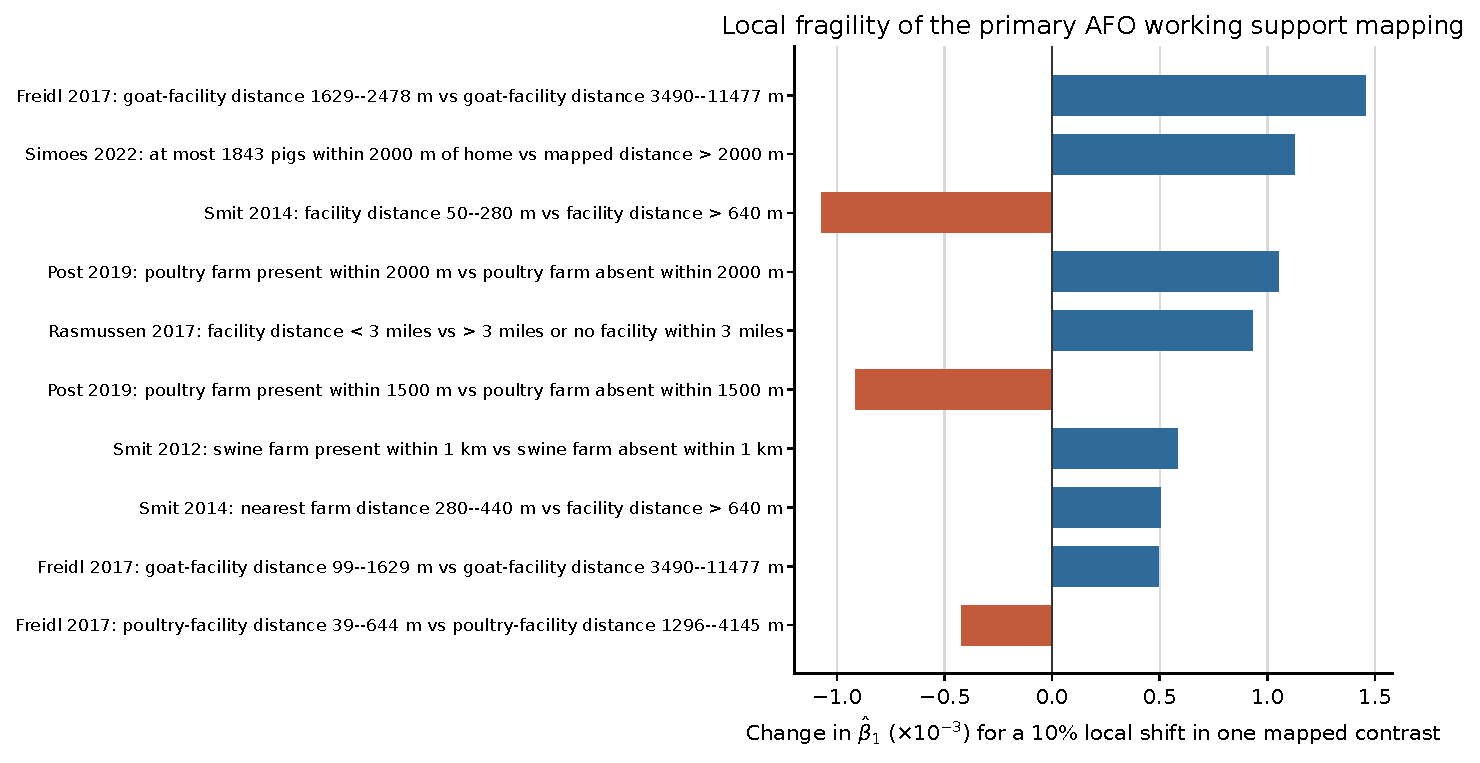
\includegraphics[width=0.98\textwidth]{images/Support_mapping_fragility.pdf}
\caption{Local fragility of the primary eight-study AFO working support-to-design mapping. Each bar is the
change in the pooled slope after a first-order 10\% perturbation of one mapped
interval contrast, holding all other mapped contrasts and reported outcomes
fixed. The ten largest absolute changes are displayed; exact point-to-point
contrasts are excluded because their design values require no interval mapping.}
\label{fig:supp_fragility}
\end{figure}

\begin{landscape}
\pdfpageattr{/Rotate 90}
\begin{table}[p]
\centering
\scriptsize
\caption{Per-comparison audit of AFO support mappings under the primary regional Gamma distributions.}\label{tab:supp_support_audit}
\resizebox{\linewidth}{!}{%
\begin{tabular}{llclllrlrr}
\toprule
Study & Region & Map & Role & Comparison support & Reference support & $d_{\max}$ & Source of finite maximum & $\mu(A)$ & $\mu(B)$ \\
\midrule
Rasmussen & PA & T1 & Explicit OR & $(0.00,3.00]$ & $(3.00,40.00]$ & 40.00 & Source graph label & 1.77 & 6.04 \\
Smit 2014 & Netherlands & T2 & Buffer OR & $(0.00,0.31]$ & $(0.31,15.00]$ & 15.00 & Same regional source & 0.20 & 0.70 \\
Smit 2014 & Netherlands & T1 & Explicit OR & $(0.27,0.40]$ & $(0.40,15.00]$ & 15.00 & Same study/source maximum & 0.34 & 0.77 \\
Smit 2014 & Netherlands & T1 & Explicit OR & $(0.18,0.27]$ & $(0.40,15.00]$ & 15.00 & Same study/source maximum & 0.23 & 0.77 \\
Smit 2014 & Netherlands & T1 & Explicit OR & $(0.03,0.18]$ & $(0.40,15.00]$ & 15.00 & Same study/source maximum & 0.13 & 0.77 \\
Smit 2012 & Netherlands & T2 & Buffer OR & $(0.00,0.62]$ & $(0.62,15.00]$ & 15.00 & Source graph label & 0.36 & 0.95 \\
Freidl 2017 & Netherlands & T2 & Buffer OR & $(0.00,0.62]$ & $(0.62,7.46]$ & 7.46 & Reported category maximum & 0.36 & 0.95 \\
Freidl 2017 & Netherlands & T2 & Buffer OR & $(0.00,0.93]$ & $(0.93,7.46]$ & 7.46 & Reported category maximum & 0.47 & 1.23 \\
Freidl 2017 & Netherlands & T2 & Buffer OR & $(0.00,0.31]$ & $(0.31,7.46]$ & 7.46 & Reported category maximum & 0.20 & 0.70 \\
Freidl 2017 & Netherlands & T1 & Explicit OR & $(0.57,0.81]$ & $(0.81,2.58]$ & 7.46 & Reported category maximum & 0.68 & 1.11 \\
Freidl 2017 & Netherlands & T1 & Explicit OR & $(1.54,2.17]$ & $(2.17,7.13]$ & 7.46 & Reported category maximum & 1.74 & 2.43 \\
Freidl 2017 & Netherlands & T1 & Explicit OR & $(0.40,0.57]$ & $(0.81,2.58]$ & 7.46 & Reported category maximum & 0.48 & 1.11 \\
Freidl 2017 & Netherlands & T1 & Explicit OR & $(1.01,1.54]$ & $(2.17,7.13]$ & 7.46 & Reported category maximum & 1.20 & 2.43 \\
Freidl 2017 & Netherlands & T1 & Explicit OR & $(0.02,0.40]$ & $(0.81,2.58]$ & 7.46 & Reported category maximum & 0.26 & 1.11 \\
Freidl 2017 & Netherlands & T1 & Explicit OR & $(0.06,1.01]$ & $(2.17,7.13]$ & 7.46 & Reported category maximum & 0.49 & 2.43 \\
Freidl 2017 & Netherlands & T2 & Buffer OR & $(0.00,1.24]$ & $(1.24,7.46]$ & 7.46 & Reported category maximum & 0.53 & 1.52 \\
Schultz 2019 & Wisconsin & T1 & Point OR & $\{1.00\}$ & $\{5.00\}$ & --- & Not required & 1.00 & 5.00 \\
Schultz 2019 & Wisconsin & T1 & Point OR & $\{1.50\}$ & $\{5.00\}$ & --- & Not required & 1.50 & 5.00 \\
Schultz 2019 & Wisconsin & T1 & Point OR & $\{2.00\}$ & $\{5.00\}$ & --- & Not required & 2.00 & 5.00 \\
Schultz 2019 & Wisconsin & T1 & Point OR & $\{2.50\}$ & $\{5.00\}$ & --- & Not required & 2.50 & 5.00 \\
Schultz 2019 & Wisconsin & T1 & Point OR & $\{3.00\}$ & $\{5.00\}$ & --- & Not required & 3.00 & 5.00 \\
Post 2019 & Netherlands & T2 & Buffer OR & $(0.00,0.31]$ & $(0.31,7.46]$ & 7.46 & Source descriptive plot & 0.20 & 0.70 \\
Post 2019 & Netherlands & T2 & Buffer OR & $(0.00,0.62]$ & $(0.62,7.46]$ & 7.46 & Source descriptive plot & 0.36 & 0.95 \\
Post 2019 & Netherlands & T2 & Buffer OR & $(0.00,0.93]$ & $(0.93,7.46]$ & 7.46 & Source descriptive plot & 0.47 & 1.23 \\
Post 2019 & Netherlands & T2 & Buffer OR & $(0.00,1.24]$ & $(1.24,7.46]$ & 7.46 & Source descriptive plot & 0.53 & 1.52 \\
Son 2021 & NC & T2 & Buffer OR & $(0.00,3.11]$ & $(3.11,43.00]$ & 43.00 & Source graph label & 1.89 & 10.76 \\
Son 2021 & NC & T2 & Buffer OR & $(0.00,6.21]$ & $(6.21,43.00]$ & 43.00 & Source graph label & 3.53 & 13.15 \\
Son 2021 & NC & T2 & Buffer OR & $(0.00,9.32]$ & $(9.32,43.00]$ & 43.00 & Source graph label & 4.92 & 15.83 \\
Son 2021 & NC & T2 & Buffer OR & $(0.00,12.43]$ & $(12.43,43.00]$ & 43.00 & Source graph label & 6.06 & 18.63 \\
Simoes 2022 & Netherlands & T2 & HR/count & $(0.00,0.31]$ & $(0.31,10.00]$ & 10.00 & Netherlands proxy region & 0.20 & 0.70 \\
Simoes 2022 & Netherlands & T2 & HR/count & $(0.00,0.62]$ & $(0.62,10.00]$ & 10.00 & Same study/source maximum & 0.36 & 0.95 \\
Simoes 2022 & Netherlands & T2 & HR/count & $(0.00,0.93]$ & $(0.93,10.00]$ & 10.00 & Same study/source maximum & 0.47 & 1.23 \\
Simoes 2022 & Netherlands & T2 & HR/count & $(0.00,1.24]$ & $(1.24,10.00]$ & 10.00 & Same study/source maximum & 0.53 & 1.52 \\
\bottomrule
\end{tabular}}
\par\smallskip
{\footnotesize T1 denotes an explicit support pair and T2 a proxy support
mapping. Role identifies restriction eligibility: Explicit OR and Point OR
records enter both restrictions, Buffer OR records enter the OR-only
restriction but not the explicit-support restriction, and HR/count records
enter only the primary working analysis.}
\end{table}
\end{landscape}
\pdfpageattr{}

\clearpage
{\sloppy\printbibliography}
\end{document}
